 \documentclass[conference]{IEEEtran}
\IEEEoverridecommandlockouts
% The preceding line is only needed to identify funding in the first footnote. If that is unneeded, please comment it out.
\usepackage{cite}
\usepackage{amsmath,amssymb,amsfonts}
\usepackage{algorithmic}
\usepackage{graphicx}
\usepackage{textcomp}
\usepackage{xcolor}
\usepackage{booktabs}
\usepackage{array}
\usepackage{adjustbox}
\usepackage[hidelinks]{hyperref}


\renewcommand{\arraystretch}{1.5}
\usepackage{makecell}
\def\BibTeX{{\rm B\kern-.05em{\sc i\kern-.025em b}\kern-.08em
    T\kern-.1667em\lower.7ex\hbox{E}\kern-.125emX}}
\begin{document}

\title{Plant Disease Detection Using Machine Learning: A Comparative Study of various plant Leaf Diseases\\
{\footnotesize \textsuperscript{}}
\thanks{}
}

\author{
    \IEEEauthorblockN{Vipin Jain}
    \IEEEauthorblockA{
        \textit{VIT Bhopal University} \\
        Sehore, Madhya Pradesh \\
        er.vipinjain@gmail.com\\
        ORCID:0000-0002-0099-3933
    }
    \and
    \IEEEauthorblockN{Riddhika Tripathi}
    \IEEEauthorblockA{
    School of Computer Science Engineering\\
        \textit{VIT Bhopal University} \\
        Sehore, Madhya Pradesh \\
        riddhikatripathi2004@gmail.com
    }
    \and
    \IEEEauthorblockN{Devanshee Shukla}
    \IEEEauthorblockA{
    School of Computer Science Engineering\\
        \textit{VIT Bhopal University} \\
        Sehore, Madhya Pradesh \\
        devansheeshukla2022@vitbhopal.ac.in
    }
}


\maketitle

\begin{abstract}
A vast number of plant pathogens from viroid’s of a few hundred nucleotides to higher plants cause diseases in our crops. Their effects range from mild symptoms to catastrophes in which large areas planted to food crops are destroyed. Plant diseases significantly impact agricultural productivity, necessitating efficient detection methods to mitigate crop losses. Plant pathogens are difficult to control because their populations are variable in time, space, and genotype. Most insidiously, they evolve, often overcoming the resistance that may have been the hard-won achievement of the plant breeder. In order to combat the losses they cause, it is necessary to define the problem and seek remedies. Our paper explores the application of machine learning techniques for detecting and classifying diseases in various plant leaves, this paper presents the stages of general plant diseases detection system and comparative study on machine learning classification techniques for plant disease detection. Machine learning methods can be used for diseases identification because it mainly apply on data themselves and gives priority to outcomes of certain task. In this survey it observed that the Convolutional Neural Network gives high accuracy and detects more diseases of multiple crops.
Using the ResNet18 model, the study detected and classified plant illnesses across 39 classes with an overall accuracy of 89.78\%. 




\end{abstract}

\textbf{\small{\textbf{Keywords- Conventional Neural Network, Machine learning methods, plant leaves.}}
}

\section{\textbf{Introduction}}
In India, Agriculture plays an essential role because of the rapid growth of population and increased demand for food. Therefore, it leads to increase in crop yield. Agriculture provides food to all the human beings even in case of rapid increase in the population. Just like human health plants health can also be affected by several diseases. In economic terms, annual losses in food, fibre and ornamental production systems caused by plant pests and diseases are estimated in the hundreds of billions of dollars \cite{r3}. These diseases are caused by fungi or fungal- like orgasms. However, other serious diseases of food and feed crops are caused by viral and bacterial organisms \cite{r4}. Some of the diseases may be of spreadable nature, meaning they may spread from one plant to other hence needing to be identified and taken care of timely. It’s very challenging job to detect disease in plants in very
 early stages. Some of the common symptoms of disease in plants disease are Leaf rust (common leaf rust in corn), Stem rust (wheat stem rust), Sclerotinia (white mold), Powdery mildew, Birds- eye spot on berries (anthracnose), Damping off of seedlings (phytophthora), Leaf spot (septoria brown spot), Chlorosis (yellowing of leaves) . In this era of technology and automation it is not very efficient approach, it would be much better if we have an automated system which detects disease in plants automatically. There is much research already done to fill this purpose; most of them utilize traditional machine learning approaches \cite{r5}. The purpose of this study is to create such automated system for detecting diseases in plants by using deep learning technique. Our system just like other previous researches utilizes images of plants leaves to detect disease in plants. Plant disease detector is computer vision based automated plant disease diagnostic system which utilizes machine learning techniques to correctly identify disease and healthy plants also the type of disease . For achieving so, deep learning networks for images like Convolution neural network (CNN) can be utilized. In our provided paper we will be using ResNet18, that is a CNN pertained model. The CNN based network can be trained for detecting disease in plants by providing huge amount of images of healthy and sick plants and trained model in future can be used to predict the disease in plants by images of plants leaves.
\begin{figure}
    \centering
    
\includegraphics[width=1\linewidth]{paperflow.drawio.png}
    \caption{Organization of paper}
    \label{fig:enter-label}
\end{figure}
\subsection{\textbf{Novelty of proposed work}}

This paper addresses current constraints in plant disease identification by using a unique mix of customised pre-processing approaches and deep learning methodology. In contrast to many other studies that use ordinary CNNs, this study optimises performance on the Plant Village dataset by utilising ResNet18, a pre-trained CNN model that has been refined by transfer learning. Strongest against changes in illumination, orientation, and picture quality—variables that are frequently disregarded in conventional methods— is ensured by integrating data augmentation techniques including gamma correction, PCA colour augmentation, and noise injection. The approach is more broadly applicable when a balanced dataset with 39 classes—including both healthy and sick leaves—is used. Using weighted loss functions and focused feature extraction, this approach also detects and corrects visually comparable illness patterns and class imbalances. The investigation also suggests potential improvements, such as the addition of multispectral imaging and explain ability tools (like Grad-CAM), laying the groundwork for applications that are easier to understand and scale. This all- encompassing strategy places the study as a major advancement in the development of precise, effective, and real-time plant disease detection systems, especially for agricultural environments with limited resources.

\section{\textbf{Literature Review}}
Since plant diseases significantly impact agriculture, extensive research on their detection and diagnosis is encouraged. Early research focused on traditional machine learning (ML) approaches that were largely based on textbooks on abstraction and AI. For example, Shruti et al.  reviewed classification methods for plant disease detection, highlighting the limitations of traditional machine learning in terms of scalability and automatic feature representation. This process is time-consuming and inefficient when dealing with complex disease data. Ferentinos \cite{r6} demonstrated the effectiveness of convolutional neural networks (CNNs) in automatic feature extraction and disease classification with high accuracy. This work demonstrates a major shift from manual engineering operations to fully automated systems. Ferentinos’ work demonstrated that CNNs are powerful tools for disease detection, successfully replicating the distribution across multiple plant species. \cite{r7} Later proposed the ResNet architecture, which is a success in deep learning. ResNet’s learning capabilities will reduce problems such as gradient fading, enable deep learning, and improve generalization capabilities. Recent studies such as Chohan et al. analyzed the performance of ResNet in classifying various plant diseases, highlighting its robustness and accuracy. However, these studies also face some challenges such as uneven distribution, similar symptoms, and limited data, which do not allow for wider application and development. Sengupta et al. \cite{r12} and Wang et al. \cite{r11} demonstrated the potential of adaptive learning in plant disease detection using pre-trained models. The learning curve reduces the need for large datasets while maintaining high accuracy, making it suitable for limited environments. Jia et al. \cite{r10} highlighted the role of frameworks such as Caffe in accelerating the development of deep learning models for agricultural applications. For example, Kumar et al.  evaluated the ability of the ResNet model to classify tomato diseases and noted the difficulty in distinguishing between visually overlapping diseases. These findings highlight the importance of improving data and decision-making processes to improve the performance of models for further advances. These include improved data quality, integration of multiple image formats, and better interpretation that makes models more usable and able to simulate real agricultural fields.

\begin{table}[h]
    \centering
    \caption{Summary of Approaches and Accuracies}
    \begin{tabular}{|p{2cm}|p{3cm}|p{1cm}|}
        \hline
        \textbf{Author} & \textbf{Approach} & \textbf{Accuracy (\%)} \\
        \hline
        
        Ferentinos \cite{r4} & CNN for automated feature extraction & 99.53 \\
        He et al.\cite{r2} & ResNet architecture with residual learning & 97.65 \\
        Chohan et al. \cite{r1} & ResNet for plant disease classification & 95.82 \\
        Sengupta et al. \cite{r12} & Transfer learning for resource efficiency & 94.50 \\
        Jia et al. \cite{r8} & Caffe framework for DL applications & Not Reported \\
        Kumar et al.\cite{r5}  & ResNet for tomato disease classification & 92.30 \\
        \hline
    \end{tabular}
    
    \label{tab:approaches_accuracies}
\end{table}



\section{\textbf{Methodology Used}}
Deep learning is a powerful machine learning approach which has mitigated the traditional machine learning headache of feature
engineering. It doesn’t need any domain expertise now and all credit goes to deep learning. The core of deep learning is artificial neural networks (ANN). Artificial neural networks are mathematical models that replicate with their neurons and synapses interconnecting them the general principles of brain function . To implement neural networks our research used the standard public available “Data Set with
Augmented Plant Leaves.” This collection includes photos of 39 distinct types of plant leaves from different plant species, including both healthy and damaged leaves. 61,486 photos in all, including background images, make up this collection. Additionally, the dataset contains a variety of plant illnesses, making it extremely pertinent to the issue of plant disease detection.
\begin{figure}
    \centering
    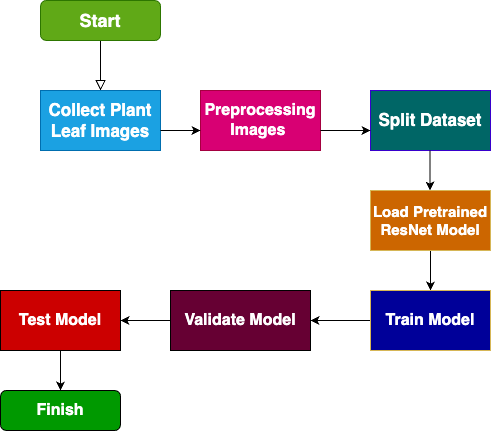
\includegraphics[width=1\linewidth]{workflow.drawio.drawio.png}
    \caption{Workflow}
    
    \label{fig:enter-label}
\end{figure}

\textit{\textbf{Workflow}}

The Plant Disease Detection Study Through the use of deep learning techniques, machine learning provides efficient illness diagnosis through an organized process. As shown in the figure 2 data collection is the first step in the process, which then moves on to categorization and outcome assessment. The process is thoughtfully planned to improve model accuracy while tackling issues including uneven datasets, noisy images, and changing illumination.
Preprocessing and data collecting are part of the first step. The Plant Village dataset, which includes 61,486 photos of 39 distinct classes—including both healthy and damaged leaves from diverse plant species—was used in this investigation. Preprocessing is done to standardize the resolution and quality of raw photographs because they might differ. To guarantee consistent input dimensions for the deep learning system, all photos are scaled to 128 by 128 pixels model of learning. Data augmentation methods such picture flipping, rotation, gamma correction, noise injection, PCA color augmentation, and scaling are also used in the work. These methods aid in the artificial expansion of the dataset, enhancing the model's capacity to identify illnesses from a variety of angles and in varying lighting circumstances.

\subsection{\textbf{ResNet18- CNN pre trained model}}\label{AA}
Nowadays deep convolutional neural networks have attained surprising outcomes in several applications. Our work is based on deep CNN with different residual networks . The ResNet is a CCN based on deep architectures that have compelling accuracy and exhibit good convergence behaviour. These models were developed by He et al \cite{r8} and have managed to win first place in both the common objects in context (COCO) and the ILSRC classification challenge in 2015. The ResNet's architecture includes a number of stacked residual units paired with a different number of layers such as 1202, 152, 101, 50, 34, 18\cite{r9}. However, the operations are bound to change, depending on the type of architecture . All the residual units are made up of pooling, convolutional, and layers. While ResNet exhibits some similarities with VGG net , it runs eight times deeper compared to VGG . The ResNet 18 is the ideal option based on its performance and depth. It is made up of a fully-connected layer with softmax, one average pooling, and five convolutional layers. The architecture of ResNet 50 packs 29 convolutional layers that are linked to the network with a fully-connected layer. In a bid to save the training time and computing resources, we chose ResNet 101, 50, 34, and 18 to help inform this study .

The Raw dataset is shown in figure 3, provides a visual representation of the many plant leaf types employed in the investigation. This picture, which shows both healthy and damaged leaves from several plant species, clearly illustrates the diversity of the dataset. One may understand the vast array of visual patterns that the model must categorize by looking at this graphic.

\subsection{\textbf{Dataset Collection}}
The dataset used , as shown in table II ,here is freely accessible Plant Leaf Augmented dataset for this study. There are 39 distinct classes of plant leaf pictures in this collection, encompassing both healthy and damaged leaves from a variety of plant species. With background pictures included, the dataset has a total of 61,486 photos. Additionally, the dataset covers a wide range of plant illnesses, making it extremely pertinent to the issue of plant disease detection.\\
By using this table you can come to know the number of images in each class. Adding up all the supports there is an average of 10,000 images approximately in the entire dataset. Fourteen different plants are available in this dataset. For every plant healthy as well as diseased images of leaves are available. Most of the images belong to Tomato and Apple and grapes plants. Least images are from Raspberry, Soybean, Blueberry, Orange and Squash class. Below image show some images of different leaves which are available in dataset.

\begin{figure}
    \centering
    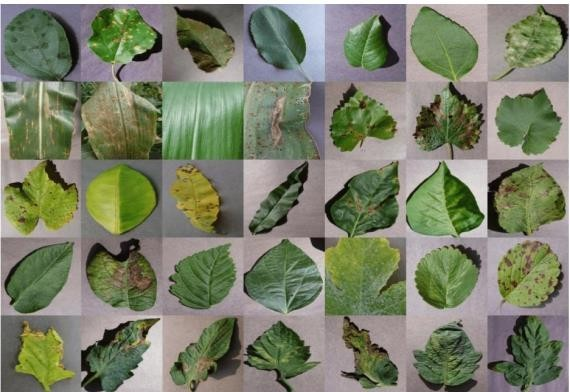
\includegraphics[width=1.0\linewidth]{sample.jpg}
    \caption{Sample of Images from Plant Village Dataset}
    \label{fig:enter-label}
\end{figure}



\subsection{\textbf{Preparation Methods}}

\begin{table}[ht]
\caption{Dataset Description}
    \centering
    \renewcommand{\arraystretch}{1.2} % Adjust row height
    \setlength{\tabcolsep}{1pt} % Adjust column spacing to reduce table width
    \begin{adjustbox}{max width=\textwidth}
    \begin{tabular}{|p{4.5cm}|c|c|c|c|}
        \hline
        \textbf{Class} & \textbf{Precision} & \textbf{Recall} & \textbf{F1-Score} & \textbf{Support} \\
        \hline
        Apple\_\_Apple\_scab & 0.9107 & 0.6800 & 0.7786 & 150 \\
        \hline
        Apple\_\_Black\_rot & 0.9282 & 0.9492 & 0.9385 & 177 \\
        \hline
        Apple\_\_Cedar\_apple\_rust & 0.9234 & 0.9188 & 0.9211 & 167 \\
        \hline
        Apple\_\_healthy & 0.8769 & 0.9012 & 0.8889 & 253 \\
        \hline
        Background\_without\_leaves & 0.9536 & 0.9840 & 0.9686 & 288 \\
        \hline
        Blueberry\_\_healthy & 0.8555 & 0.9555 & 0.9021 & 150 \\
        \hline
        Cherry\_\_Powdery\_mildew & 0.9212 & 0.9620 & 0.9412 & 158 \\
        \hline
        Cherry\_\_healthy & 0.9101 & 0.9640 & 0.9364 & 150 \\
        \hline
        Corn\_\_Cercospora\_leaf\_spot & 0.7907 & 0.8346 & 0.8119 & 163 \\
        \hline
        Corn\_\_Common\_rust & 0.9479 & 0.9479 & 0.9479 & 169 \\
        \hline
        Corn\_\_Northern\_Leaf\_Blight & 0.8357 & 0.7452 & 0.7879 & 178 \\
        \hline
        Corn\_\_healthy & 0.8945 & 0.9176 & 0.9059 & 172 \\
        \hline
        Grape\_\_Black\_rot & 0.9209 & 0.7442 & 0.8231 & 220 \\
        \hline
        Grape\_\_Esca\_Black\_Measles & 0.8421 & 0.9455 & 0.8903 & 220 \\
        \hline
        Grape\_\_Leaf\_blight & 0.9383 & 0.9383 & 0.9383 & 162 \\
        \hline
        Grape\_\_healthy & 0.9121 & 0.9764 & 0.9432 & 170 \\
        \hline
        Orange\_\_Haunglongbing\_Citrus\_ & 0.9856 & 0.9933 & 0.9894 & 899 \\
        
        greening &  &  &  & \\
        \hline
        Peach\_\_Bacterial\_spot & 0.9701 & 0.8832 & 0.9246 & 368 \\
        \hline
        Peach\_\_healthy & 0.9395 & 0.9575 & 0.9484 & 160 \\
        \hline
        Pepper\_bell\_\_Bacterial\_spot & 0.9302 & 0.7595 & 0.8363 & 148 \\
        \hline
        Pepper\_bell\_\_healthy & 0.9149 & 0.9111 & 0.9130 & 174 \\
        \hline
        Potato\_\_Early\_blight & 0.8204 & 0.9648 & 0.8863 & 142 \\
        \hline
        Potato\_\_Late\_blight & 0.8800 & 0.8250 & 0.8519 & 160 \\
        \hline
        Potato\_\_healthy & 0.9044 & 0.9595 & 0.9311 & 154 \\
        \hline
        Raspberry\_\_healthy & 0.9681 & 0.8765 & 0.9204 & 160 \\
        \hline
        Soybean\_\_healthy & 0.9699 & 0.9733 & 0.9715 & 860 \\
        \hline
        Squash\_\_Powdery\_mildew & 0.9739 & 0.9503 & 0.9620 & 278 \\
        \hline
        Strawberry\_\_Leaf\_scorch & 0.9755 & 0.9575 & 0.9664 & 170 \\
        \hline
        Strawberry\_\_healthy & 0.8982 & 0.9494 & 0.9231 & 158 \\
        \hline
        Tomato\_\_Bacterial\_spot & 0.8572 & 0.8172 & 0.8367 & 212 \\
        \hline
        Tomato\_\_Early\_blight & 0.8750 & 1.0000 & 0.9333 & 160 \\
        \hline
        Tomato\_\_Late\_blight & 0.7103 & 0.8444 & 0.7719 & 90 \\
        \hline
        Tomato\_\_Leaf\_Mold & 0.8154 & 0.7218 & 0.7653 & 147 \\
        \hline
        Tomato\_\_Septoria\_leaf\_spot & 0.7143 & 0.6143 & 0.6600 & 140 \\
        \hline
        Tomato\_\_Spider\_mites & 0.7931 & 0.6129 & 0.6923 & 124 \\
        \hline
        Tomato\_\_Target\_Spot & 0.7551 & 0.6789 & 0.7149 & 76 \\
        \hline
        Tomato\_\_Tomato\_Yellow\_Leaf\_Curl & 0.9395 & 0.9744 & 0.9567 & 1177 \\
        \_Virus & & & & \\
        \hline
        Tomato\_\_Tomato\_mosaic\_virus & 0.9344 & 0.8415 & 0.8854 & 207 \\
        \hline
        Tomato\_\_healthy & 0.9783 & 0.9171 & 0.9468 & 338 \\
        \hline
        \textbf{Accuracy} & \multicolumn{4}{c|}{0.8978} \\
        \hline
        \textbf{Macro Avg} & 0.8829 & 0.8756 & 0.8738 & 0.8978 \\
        \hline
        \textbf{Weighted Avg} & 0.8997 & 0.8978 & 0.8924 & 0.8978 \\
        \hline
    \end{tabular}
    \end{adjustbox}
    
    \label{tab:metrics}
\end{table}


\begin{itemize}
    \item Image Resizing: To expedite the model training process while preserving key characteristics, the pictures were downsized to 128x128 pixels.
\end{itemize}
\begin{itemize}
    \item Data Augmentation: We employed a number of data augmentation approaches to artificially expand the dataset's size and variety because, despite its size, it is still prone to class imbalances. Among these augmentations are:
\end{itemize}
\begin{figure}
    \centering
    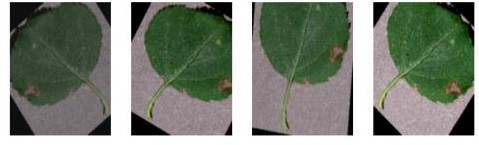
\includegraphics[width=1.0\linewidth]{smp1.jpg}
    \caption{Augmentation demonstration}
    \label{fig:enter-label}
\end{figure}

\begin{enumerate}
    \item Image Flipping: This technique simulates several viewpoints by flipping an image horizontally.
    \item Gamma Correction: Used to regulate brightness in response to varying lighting conditions.
    \item Noise Injection: Noise is added to create the illusion of noisy or low-quality photographs.
    \item PCA Colour Augmentation: Used to provide colour diversity, this technique increases resilience to various circumstances.
    \item Rotation: To replicate different plant leaf orientations, random rotations are used.
    \item Scaling: To deal with the variations in plant leaf sizes in the photos, scaling was used.\\
    Feature Extraction: A convolutional neural network (CNN) pre-trained on the ImageNet dataset, ResNet18, was used to extract features.To diagnose the plant leaf diseases, transfer learning was used, which involved freezing the layers of the pre-trained model and fine-tuning the final fully linked layers. While the final layers are modified to categorise the particular plant diseases, the pre-trained weights from ImageNet assist the model in learning key characteristics that are frequently found in real photos, such as edges, textures, and patterns.
\end{enumerate}

\subsection{\textbf{Model Description}}
\begin{table}[h]
\caption{ResNet18 Parameters and values}
    \centering
    \renewcommand{\arraystretch}{1.5}  % Adjust row height for vertical centering
    \begin{tabular}{|>{\centering\arraybackslash}p{2cm}|>{\centering\arraybackslash}p{3cm}|>{\centering\arraybackslash}p{2.5cm}|}
    \hline
    \textbf{Parameter} & \textbf{Description} & \textbf{Value/Notes} \\ \hline
    Input Image Size & Size of the input images fed to the ResNet18 & 224 x 224 pixels (default for ResNet18) \\ \hline
    Number of Layers & Total layers in the ResNet18 architecture & 18 classes \\ \hline
    Pre-trained Weights & Weights used for initialization & ImageNet (optional for transfer learning) \\ \hline
    Number of Parameters & Total trainable parameters & ~11.7 million \\ \hline
    Batch Size & Number of images processed in a single forward/backward pass & Typically 16, 32, or 64 (depends on computational resources) \\ \hline
    Learning Rate & Step size for updating weights during training & Commonly between 0.001 and 0.0001 (with learning rate decay) \\ \hline
    Optimizer & Algorithm used to minimize the loss function & Adam or SGD (with momentum) \\ \hline
    Loss Function & Function to evaluate the error during training & Cross-Entropy Loss (suitable for multi-class classification) \\ \hline
    Activation Function & Non-linearity used between layers & ReLU \\ \hline
    Pooling Layer & Type of pooling used & Global Average Pooling (before FC layer) \\ \hline
    Number of Epochs & Total iterations over the entire dataset & 20-50 epochs (or until convergence) \\ \hline
    Fine-Tuned Layers & Layers adjusted for the dataset-specific task & Fully connected layers fine-tuned for classification \\ \hline
                               Evaluation Metrics & Metrics used to assess the model’s performance & Precision, Recall, F1-Score, Accuracy \\ \hline
    Framework/Library & Deep learning library used for implementation & PyTorch, TensorFlow, or Keras \\ \hline
    \end{tabular}
    \label{tab:cnn_parameters}
\end{table}

For this test, we used the deep residual network ResNet18, which has demonstrated exceptional performance in picture classification tests. A fully connected classification layer comes after several convolutional layers in the ResNet18 architecture. This model was selected because:
\begin{itemize}
    \item Pre-trained Weights: By using ImageNet's pre- trained weights, the model gains from past experience and improves its ability to generalise with less data.
    \item Residual Blocks: ResNet's residual blocks facilitate deep network training by facilitating gradient passage through the network, hence mitigating the vanishing gradient issue.The PyTorch framework, which offers an adaptable and effective platform for deep learning applications, was used to create the model.
\end{itemize}

\section{\textbf{Results}}
This study shows the importance of plant disease detection in these days. This model were developed using Deep Learning in python.The model performed well in identifying plant illnesses and healthy conditions across 38 classes, with an overall accuracy of 89.78\%. Its efficacy is demonstrated by metrics like a weighted F1-score of 0.8924 and a macro F1- score of 0.8784, especially for well-represented classes like Orange	Haunglongbing and Soybean	healthy. Flipping, rotation, and gamma correction are examples of data augmentation approaches that improved the model's resilience to changes in viewpoint, illumination, and orientation. ResNet18's transfer learning made use of pre-trained features, which ensured effective training while lowering the requirement for large amounts of labelled data. However, because of class imbalance, under- represented classes—like Pepper, Bell, and Healthy—performed worse, indicating the necessity of weighted loss functions or dataset balancing. Additionally, difficulties in differentiating visually identical illnesses were noted, highlighting the usefulness of multispectral imaging or domain-specific characteristics.
Although more improvements in explainability, dataset diversity, and regional adaptability might increase the model's usefulness in actual agricultural contexts, its computing efficiency and resilience to a variety of situations make it appropriate for deployment.

The resilience of the model was greatly enhanced by data augmentation methods such PCA colour augmentation, gamma correction, scaling, random rotations, horizontal flips, and noise injection. The model was able to manage a variety of orientations, viewpoints, lighting conditions, and picture quality thanks to these strategies that mimicked real-world differences. Furthermore, the model was able to utilise pre- existing low- and mid-level picture characteristics using transfer learning with ResNet18 pre- trained on the ImageNet dataset, which lessened the need for extensive labelled datasets. Task- specific learning was made possible without overfitting by fine-tuning just the last few layers of the previously trained model, guaranteeing effective training.

\begin{figure}
    \centering
    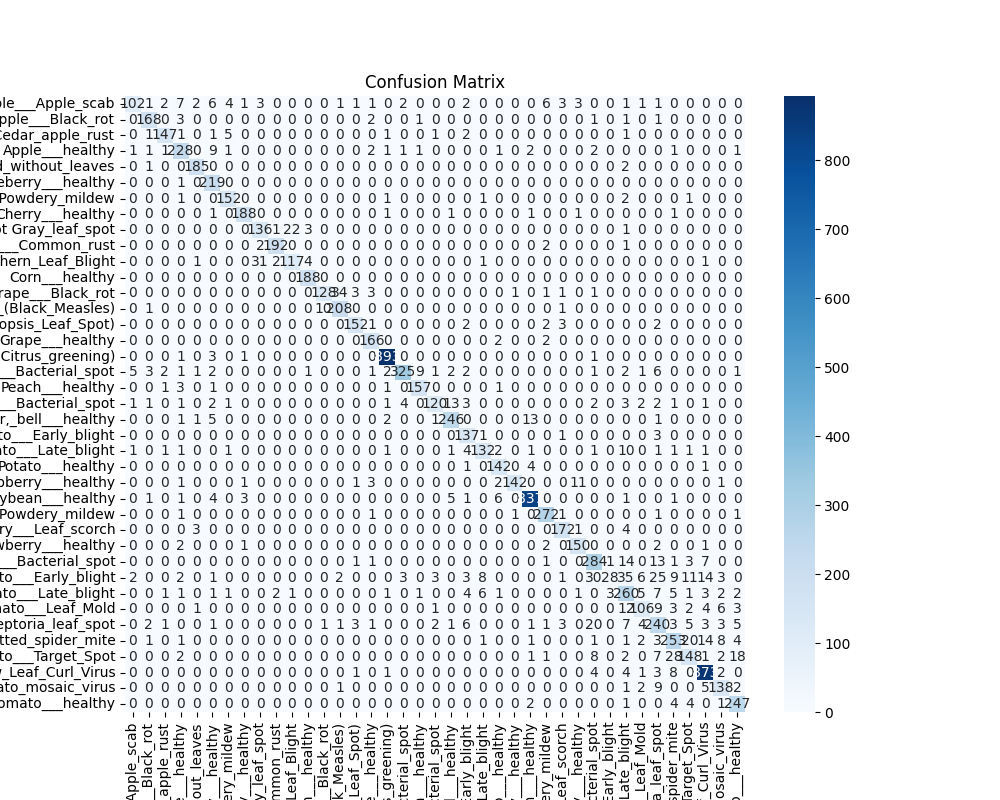
\includegraphics[width=1\linewidth]{confusion_matrix.png}
    \caption{Confusion Matrix of proposed work}
    \label{fig:enter-label}
\end{figure}
The complete dataset was used to assess the model's performance, with the confusion matrix providing valuable insights into the classification accuracy and trends in classifications. 
The computational efficiency of the modelmodelmodel makes it suitable for din devices limited in resources, allowing real-time diagnosis of plant disease disease disease in agricultural settings. However, further improvements could include incorporating explainability tools, such as Grad- CAM, to visualize the regions of interest in the images that influence predictions. Additionally, expanding the dataset to include region-specific data and environmental factors could improve its generalizability and practical utility. Overall, the model demonstrates strong potential for assisting farmers and agricultural professionals in disease detection, with opportunities for refinement to maximize its effectiveness in diverse real-world scenarios.


\begin{figure}
    \centering
    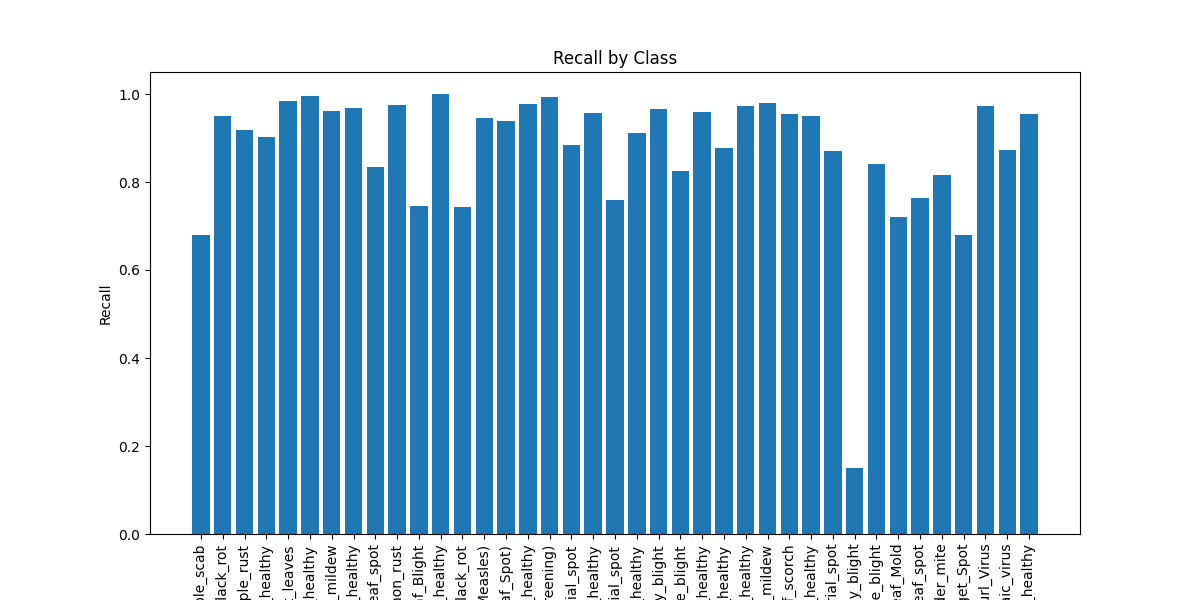
\includegraphics[width=1\linewidth]{recall_plot.png}
    \caption{Recall by class}
    \label{fig:enter-label}
\end{figure}
\begin{figure}
    \centering
    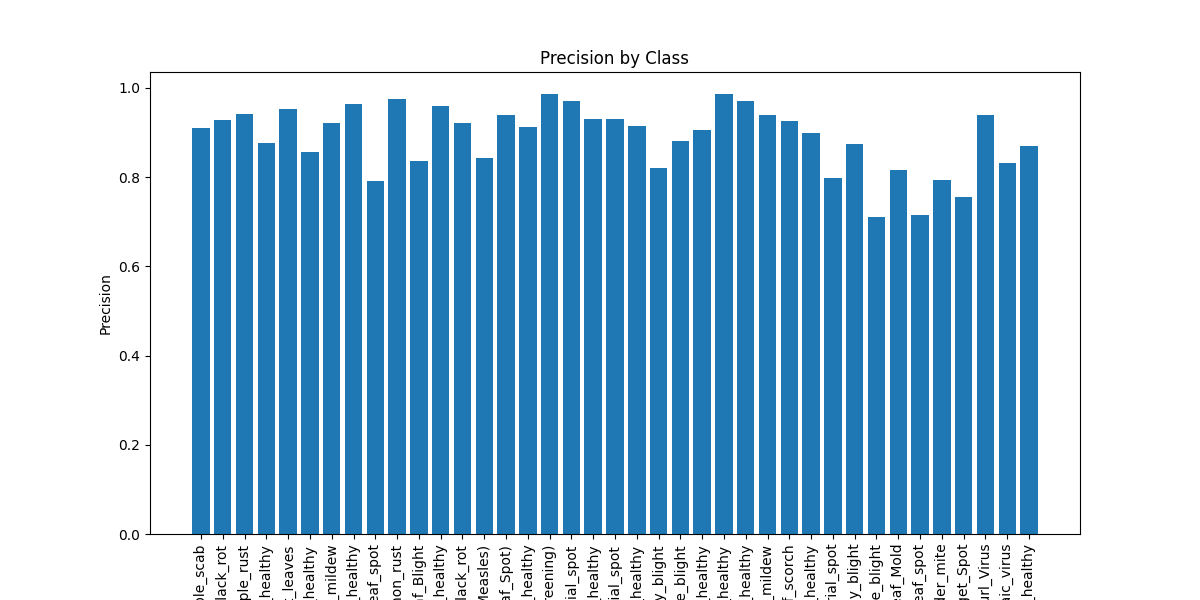
\includegraphics[width=1\linewidth]{precision_plot.png}
    \caption{Precession by class}
    \label{fig:enter-label}
\end{figure}
\begin{figure}
    \centering
    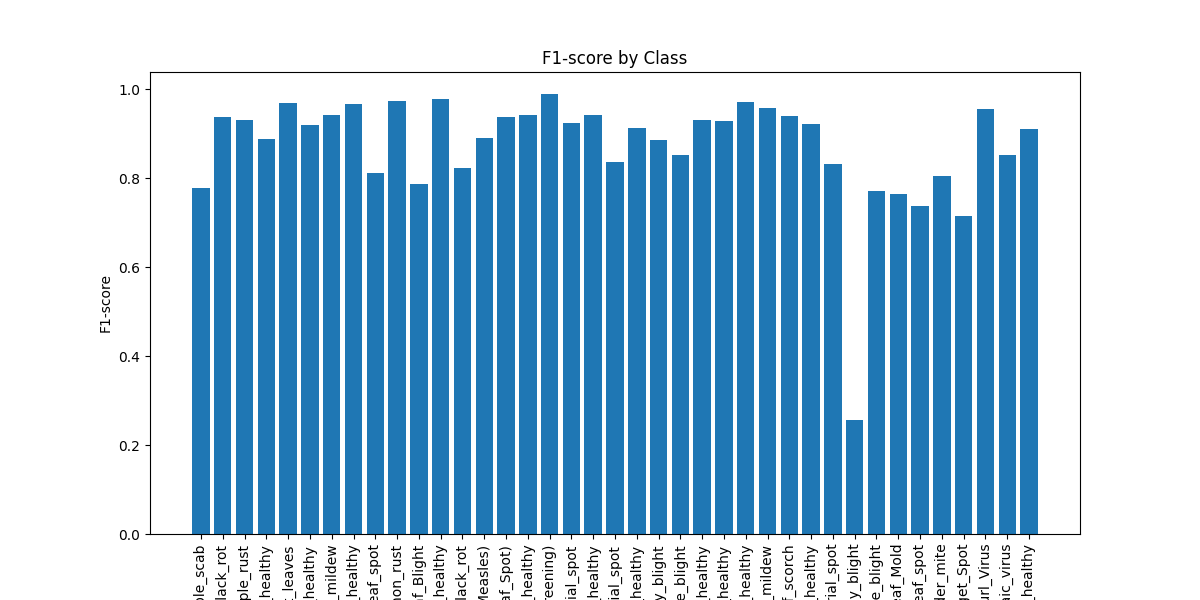
\includegraphics[width=1\linewidth]{f1-score_plot.png}
    \caption{F1-score by class}
    \label{fig:enter-label}
\end{figure}

\vspace{1cm}


\section{\textbf{Conclusion}}

The model excels at recognizing well-represented classes such as Orange Huanglongbing and Soybean healthy, with minimal misclassification in these categories, as evidenced by their high F1\-scores, accuracy, and precision. However, certain visually similar classes, like Potato Early\_blight and Potato Late\_blight, show significant misclassifications due to overlapping visual features, such as leaf discoloration and texture variations. This issue is further complicated by the class imbalance in the dataset, as seen in the higher misclassification rates for under-represented classes like Pepper bell healthy.

Despite these challenges, the model achieved a high overall accuracy of 89.78\%, indicating its suitability for real-world plant disease diagnostic applications. The use of data augmentation techniques, such as flipping, rotation, and scaling, strengthened the model by improving its robustness against changes in viewpoint, orientation, and size. Leveraging ResNet18 through transfer learning ensured both high accuracy and computational efficiency. The confusion matrix highlights the need for addressing misclassification patterns through techniques like weighted loss functions, balanced datasets, or advanced feature extraction methods. When combined with explainability tools like Grad-CAM, which highlights focus areas in images, these improvements could significantly enhance the model's performance.

Looking ahead, there are several important avenues for improving the model's performance and application. One key area is enhancing the performance of under-represented classes, which may be addressed by cutting-edge techniques like Generative Adversarial Networks (GANs) and oversampling strategies such as SMOTE. Incorporating multi-spectral and hyper-spectral imaging data could further refine the model's ability to distinguish between visually similar diseases by providing additional feature extraction from beyond the visible spectrum.

Improving model interpretability with tools like Grad-CAM or SHAP could make predictions more transparent, helping users understand the factors influencing the results. Furthermore, model optimization techniques, such as pruning or quantization, may enable real-time deployment on edge devices like smartphones or IoT-enabled cameras, expanding access to plant disease detection for farmers. Enlarging the dataset to include regional variations in plant diseases and incorporating multi-disease detection capabilities could further improve the model's generalizability.

\textbf{{
\section{\textbf{ Future Work Scope}}
}}

Integrating environmental variables like temperature, humidity, and soil quality with image data could lead to a more comprehensive diagnostic system that supports proactive disease prevention. Cross-domain learning, leveraging datasets from related fields like weed or pest detection, could broaden the model’s applicability. Additionally, automating data collection through drones or robotic devices could expedite the compilation of diverse datasets while reducing manual labor. Finally, integrating the model with cloud computing and IoT platforms could enable seamless data collection, analysis, and real-time insights, facilitating widespread agricultural applications.

Together, these advancements would significantly enhance the effectiveness of AI-driven agricultural tools, contributing to global efforts to improve crop productivity and health.

\bibliographystyle{IEEEtran}
\bibliography{bibfile.bib}



\vspace{12pt}

\end{document}
